% QDots
%  Created by Syed Ali Moeed Tirmzi May 29, 2015

% %%   PREAMBLE   %%%

% PREPRINT
%\RequirePackage[displaymath,mathlines]{lineno}  % implement numbered lines
%\documentclass[aps,prl,preprint,citeautoscript,superscriptaddress,byrevtex,nofootinbib]{revtex4}
%\documentclass[aps,prl,preprint,citeautoscript,superscriptaddress,endfloats*,byrevtex,nofootinbib]{revtex4}

% GALLEY
%\RequirePackage[displaymath,mathlines]{lineno}  % implement numbered lines -- pagewise for two-column mode
%\documentclass[10pt,aps,prl,twocolumn,galley,citeautoscript,superscriptaddress,byrevtex,nofootinbib,nobalancelastpage,floatfix]{revtex4}

% TWO COLUMN
%\RequirePackage[displaymath,mathlines,pagewise]{lineno}  % implement numbered lines -- pagewise for two-column mode
%\RequirePackage[displaymath,mathlines]{lineno}  % implement numbered lines -- pagewise for two-column mode
\documentclass[aps,prl,twocolumn,citeautoscript,superscriptaddress,byrevtex,nofootinbib,nobalancelastpage,floatfix]{revtex4}

% PACKAGES
\usepackage{siunitx}    % package for \meter etc
\usepackage[pdftex]{graphicx}         % \includegraphics{}
\usepackage{fancyhdr}                 % \pagestyle{fancy}, \rhear{}, rfoo{}
\usepackage{amsmath}                  % \pmatrix{}, etc...
\usepackage{bm}                       % need for bold greek letters
\usepackage[letterpaper,
    margin=1.0in,
    includehead,
    includefoot,
    headsep=11pt]{geometry}   % large margins
\usepackage[colorlinks=true,
    citecolor=red,
    linkcolor=blue,
    urlcolor=blue,
    pagebackref=false]{hyperref}
\usepackage{mciteplus}
\usepackage{bm}         % bold math
\usepackage{natbib}  % bibliography
%\RequirePackage{lineno}
                                    
% FONTS

% Computer Modern is the default LaTeX font.
% Uncomment one of the lines below to try another font.
% PRL actually appears to use a font closet to Times.
% \usepackage{times}     % ~not~ computer modern fonts
\usepackage{palatino}  % ~not~ computer modern fonts

% FORMATTING OPTIONS

\lefthyphenmin=3           % Fix LaTeX hyphenation
\righthyphenmin=4          % Fix LaTeX hyphenation
%\setlength{\parskip}{6pt}  % Set paragraph spacing to be easy on the eyes

\graphicspath{
{/Users/alimoeedt/Dropbox/_JAM_FP__Tirmzi201505__Qdots_SPM__figs/}
}

% COMMANDS
\newcommand{\trimcaptionspacing}{\vspace{-0.25in}}      % include in figures to decrease the text-to-figure spacing
\newcommand{\trimcaptionspacinghalf}{\vspace{-0.10in}}  % include in figures to decrease the text-to-figure spacing
\def\bibfont{\footnotesize} % Smaller font in the bibliography

%%%%%%%%%%%%%%%%%%%%%%%%%%%%%%%%%%%%%%%%%%%%%%%%%%%%%%%
%%%%%%%%%%%%%%%%  Begin Document %%%%%%%%%%%%%%%%%%%%%%
%%%%%%%%%%%%%%%%%%%%%%%%%%%%%%%%%%%%%%%%%%%%%%%%%%%%%%%

\begin{document}

    \pagestyle{fancy}

        \lhead{\footnotesize \textsf{AUTHORS}}
        \chead{\normalsize Short title}
        \rhead{\footnotesize \textsf{\today}}
        \lfoot{}
        \cfoot{\thepage}
        \rfoot{}


    \title{QDots}

    \author{Syed Ali Moeed Tirmzi}
    \affiliation{Department of Chemistry and Chemical Biology, Ithaca, New York 14853}

    \author{John A. Marohn}
    \affiliation{Department of Chemistry and Chemical Biology, Ithaca, New York 14853}

    % LINE NUMBERING
    %\setpagewiselinenumbers
    %\modulolinenumbers[5]
    %\linenumbers

\begin{abstract}
    This is the abstract.
\end{abstract}

\date{\today}

\maketitle
\thispagestyle{fancy}


\section{Introduction}
This is the body \cite{Somebody1900}.  I do not like this silly reference.

\begin{figure}
    \label{fig:Example}
    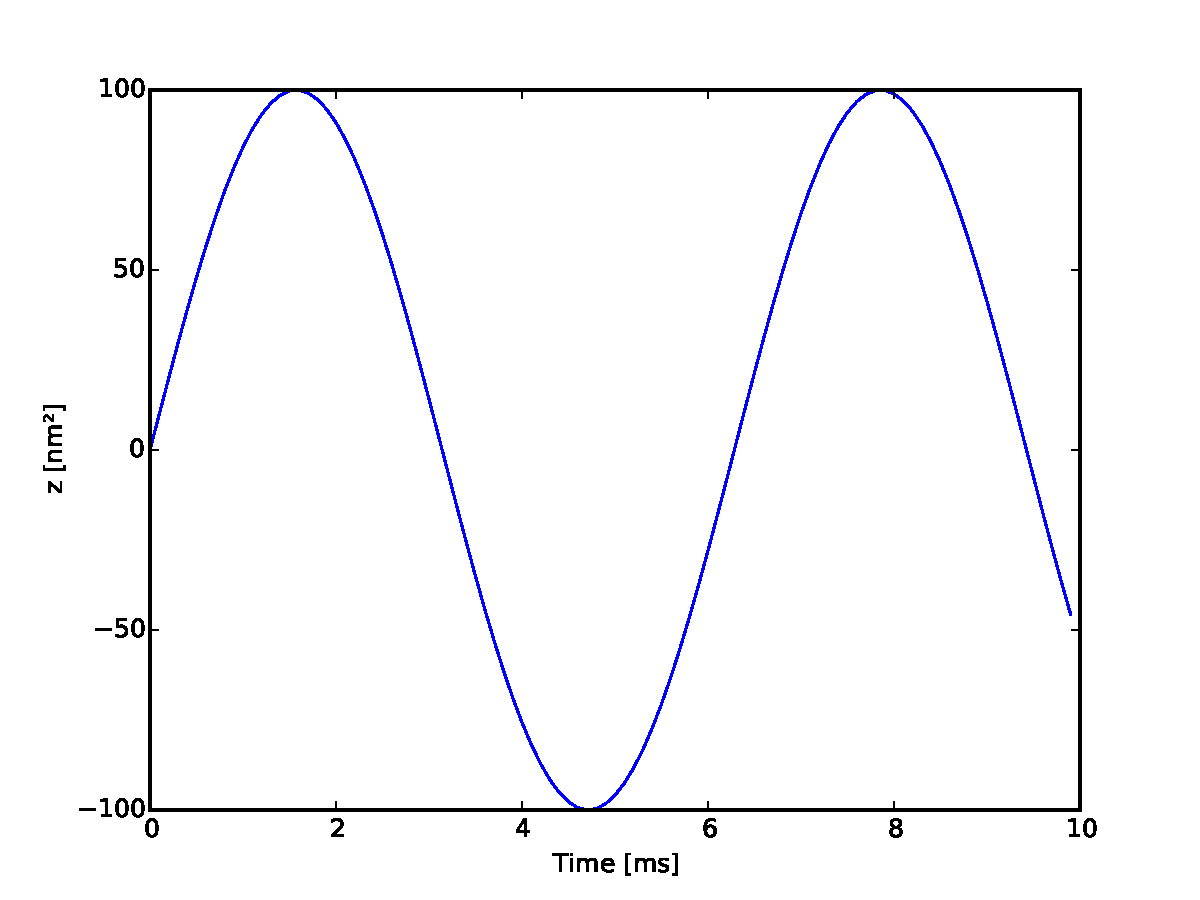
\includegraphics[width=3.1in]{figs/ex.pdf}
    \caption{Example figure}
\end{figure}


% =========================
\def\bibsection{\vspace{6pt}}
\setlength{\bibsep}{0pt}

\bibliographystyle{bst/naturemag_jm}

\bibliography{bib/Literature_Tirmzi}
\label{TheEnd}
\end{document}
